\documentclass[letterpaper, 11pt]{article}

\usepackage{lastpage, marginnote, siunitx, circuitikz, kantlipsum, hyperref, amsmath}
\def\UrlBreaks{\do\/\do-}

%\usepackage[hyphens]{url}

\usepackage{geometry}
\geometry{hscale=.6, vscale=.8, hmarginratio=2:1, vmarginratio=1:1, marginparwidth=.18\paperwidth, ignoremp}
%\geometry{marginparwidth=.1\paperwidth}

%\usepackage[T1]{fontenc}

\usepackage[explicit]{titlesec}
\titlespacing*{\section}{\dimexpr -\marginparsep-\marginparwidth}{*4}{*1}
\titleformat{\section}[runin]{\large\bfseries\titlerule[.5pt]\filright}{\makebox[1em][c]{\thesection}}{1em}{\parbox[t]{\dimexpr\marginparwidth-2em}{#1}\hskip\marginparsep\mbox{}}[\newline\vspace{-4ex}]

%\titlespacing*{\subsection}{\dimexpr -\marginparsep-\marginparwidth}{*4}{*1}
%\titleformat{\subsection}[runin]{\large\bfseries\titlerule[.5pt]\filright}{\makebox[1em][c]{\thesection}}{1em}{\parbox[t]{\dimexpr\marginparwidth-2em}{#1}\hskip\marginparsep\mbox{}}[\newline]

\usepackage{enumitem}
\newlist{steps}{enumerate}{1}
\setlist[steps]{label=Step \arabic*, font=\bfseries, leftmargin=-\marginparsep, itemindent=\marginparsep, align=right}

\usepackage{fancyhdr}
\pagestyle{fancy}
\fancyhf{}
\fancyhfoffset[lh,lf]{\dimexpr\marginparwidth+\marginparsep}
\fancyhf[lh]{UCD EEC 134}
\fancyhf[ch]{}
\fancyhf[rh]{}
%\fancyhf[lf]{left foot}
%\fancyhf[cf]{centre foot}
\fancyhf[rf]{Page \thepage /\pageref{LastPage}}
%\renewcommand{\footrulewidth}{.4pt}

%%%%%%%%%%%%%%%
%%%% Tikz definitions
%%%%%%%%%%%%%%%
%\tikzstyle{Uno}=[rectangle,fill=white,draw,line width=0.5mm]

%new commands
%display due date in red and link to the eec134-schedule.pdf document
\newcommand{\due}[1]{\href{https://github.com/ucdart/UCD-EEC134/blob/master/support/schedule/eec134-schedule.pdf}{\textcolor{red}{#1}}}

\graphicspath{{./figures/}}

\begin{document}

\title{Lab 1: Elements of Electronic Systems}
\author{Instructor: Xiaoguang ``Leo'' Liu\\lxgliu@ucdavis.edu \\
	\small \href{http://creativecommons.org/licenses/by-sa/4.0/}{CC BY-SA 4.0}}
%\date{}
\date{Last updated: \today}

\maketitle

The main objective of this lab is to understand the basic components of a typical electronic system. To this end, we will build a simple electronic system shown in Fig.~\ref{fig:lab1-system}. In this system, we will use a micro-controller and a digital-to-analog converter (DAC) to generate a triangle wave. This triangle wave signal will be low pass filtered and digitized by an analog-to-digital converter (ADC) whose output will be sent to a computer for analysis and display.

Although this system may seem rather useless, it does serve the purpose of introducing the basic concepts and skills in building an embedded system that needs to interface with the analog world. In addition, some of the components in this system will become useful in later labs. 

\begin{figure}[h]
	\centering
	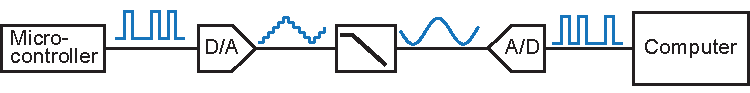
\includegraphics{lab1-system}
	\caption{Lab 1 electronic system.}
	\label{fig:lab1-system}
\end{figure}

\section{Objectives}

\begin{enumerate}[itemsep=0.1ex]
	\item Understand the functionality and characteristics of linear and switching voltage regulators;
	\item Learn how to use simple micro-controllers, such as the Arduino Uno and the Teensy 3.1;
	\item Learn the functionality and use of DAC and ADC;
	\item Learn how to use the serial programming interface to control electronic components;
	\item Learn the basic skills of designing and laying out a printed circuit board (PCB);
	\item Learn the basic skills PCB assembly involving surface mount (SMD) components.
\end{enumerate}

%Be warned that this lab is a fairly aggressive one and it will take a lot of time for you and your group to finish all the reading, the pre-lab assignment, the actual lab, and the reports. It's a good idea to start early! And divide up tasks between group members wisely!


\newpage
\section{Prelab}
\subsection{Micro-controller}
Micro-controllers are computing systems integrated within a single package. Compared with general purpose computers, micro-controllers find widespread use in applications where low-power consumption, small physical size, low cost, and predictable response time are required. 

Traditionally, programming a micro-controller was an art that only well-trained electrical engineers can perform. This all changed with the invention of the Arduino micro-controller platform in 2005 by a group of Italian educators who were frustrated with how difficult it was to learn and use microcontrollers. They decided to develop a hardware and software platform so easy to use that even artists were able to use them. In addition, the Arduino platform is completely open source. Because of this, there has been a large number of library and add-on boards (called ``Shields'') developed and made available by the community, making it possible to build complex systems without having to reinvent the wheels. The huge popularity of the Arduino platform has motivated the development of numerous similar platfomrs with a wide spectrum of capabilities. These are the reasons that we choose to use Arduino compatible micro-controllers in this class\footnote{If you have experience using a microcontroller different than the Arduinos, you should feel free to use that platform to implement this lab; obviously you may want to make sure that you have a consensus within your group.}. We hope that even students who are not interested in embedded systems will be able to master how to use them in a relatively short of time. 

Although the focus of the EEC 134 class is on high frequency systems, you will find that micro-controllers indispensable whenever you need to control a component electronically.  

\begin{itemize}[itemsep=0.1ex]
	\item To get a quick introduction to the Arduino platform, watch Episodes 1--10 of Jeremy Blum’s ``\href{https://www.youtube.com/playlist?list=PLA567CE235D39FA84}{Tutorial Series for Arduino} ''. It is advised that you, or your group collectively, go through all of the videos in this list. 	\url{https://www.youtube.com/playlist?list=PLA567CE235D39FA84}
	
	%\item Go through Appendix A: A Teensy Primer
\end{itemize}


\subsection{Voltage regulator}
In the late 1880s, a heated battle over the best mechanism to transport electricity over long distance broke out between proponents of direct current (primarily Thomas Edison) and alternating current (primarily George Westinghouse and several European companies). History eventually settled on ac current as the preferred method for long distance distribution because of its ability to be easily transformed into high voltages to reduce resistive loss along the wires. So today we all have ac outlets at home and in the lab. However, most if not all the circuits we have studied in our curriculum are powered from dc supplies. Have you ever wondered how dc voltages are generated from an ac supply? The following videos may be instructive. Make sure you watch them carefully. 

\begin{itemize}[itemsep=0.1ex]
	\item How to build an AC-DC power supply:\\ \url{https://www.youtube.com/watch?v=cyhzpFqXwdA} 
	\item Linear voltage regulator:\\ \url{https://www.youtube.com/watch?v=GSzVs7_aW-Y}
	\item Adjustable linear voltage regulator:\\  \url{https://www.youtube.com/watch?v=IjJWWGPjc-w}
	\item Switch-mode voltage regulator:\\ \url{https://www.youtube.com/watch?v=CEhBN5_fO5o}
\end{itemize}

\subsection{DAC and ADC}

DAC and ADC are the interface between the analog and the digital world. A DAC takes digital input (``1''s and ``0''s) and convert them into an analog signal. An ADC does the just the inverse of that, converting an analog signal into a digital one. A simple DAC can be built with only resistors, such as the R-2R ladder shown in Fig.~\ref{fig:dac-adc}-a. A simple ADC is not much more complex using a linear resistor ladder integrated with comparator and decoders (Fig.~\ref{fig:dac-adc}-b)\footnote{A variety of other architectures exist for both DACs and ADCs with respective advantages and disadvantages.}

\begin{figure}[h]
	\centering
	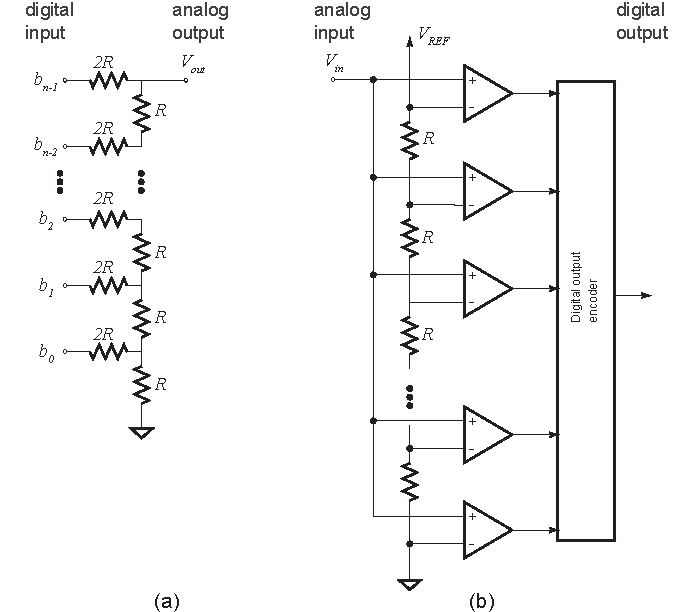
\includegraphics{dac-adc}
	\caption{(a) R-2R ladder DAC. (b) ADC using a linear string of resistors.}
	\label{fig:dac-adc}
\end{figure}


To learn more about DACs and ADCs, watch the following video and read the following documents. 

\begin{itemize}[itemsep=0.1ex]
	
	\item humanHardDrive, ``Electronics 201 -- Analog/Digital Conversion,''\\ \url{https://www.youtube.com/watch?v=cjmcAE1L6OQ}
	\item Bill McCulley, ``\href{https://github.com/ucdart/UCD-EEC134/blob/c58efc438dba2679658333c34c4a6f733f594b39/labs/lab1/references/%5BMcCulley2010%5D.DAC.Introduction.pdf}{Bridging the divide: Part I - DAC Introduction}\footnote{Following the link  will lead you to EEC134's repository on Github. If you want the actual PDF file, you can clone the entire repository to your harddrive. The file is under the foler /labs/lab1/references/.},'' National Semicondcutor, 2010
	\item Chris Pearson, ``\href{https://github.com/ucdart/UCD-EEC134/blob/e977e88aaaf67f53cd562d2a071746a38ea19aa3/labs/lab1/references/%5BPearson2012%5D.High.Speed.Analog.to.Digital.Converters.Basics.pdf}{High Speed, Digital to Analog Converters Basics},'' Texas Instruments, 2012.
	\item Mike Kester, ``\href{http://www.analog.com/media/en/training-seminars/tutorials/MT-019.pdf}{DAC Interface Fundamentals},'' Analog Devices, 2008.
	\item Chris Pearson,  ``\href{https://github.com/ucdart/UCD-EEC134/blob/da59c17c776faf159aaea506ebd87510907dc133/labs/lab1/references/%5BPearson2011%5D.High-Speed.Analog-to-Digital.Converter.Basics.pdf}{High-Speed, Analog-to-Digital Converters Basics},'' Texas Instruments, 2011.
\end{itemize}

\subsection{Serial interface}

For micro-controllers that don't have built-in DACs and/or ADCs, an external DAC/ADC IC needs to be used when conversion between analog and digital is required. Even micr-controllers with on-chip DAC/ADC may run into situations where more than conversions channels are needed. When using an external device, a digital interface for transmitting and receiving data is needed between the micro-controller and the device. 

Digital interface generally comes in two flavors: \textit{parallel} and \textit{serial}. In a parallel interface, each physical pin corresponds to one digital bit. For example, an 8-bit word would need 8 physical pins for transmission/reception. In a serial interface, the digital bits are transmitted/received sequentially in time and theoretically only two pins are needed (one for signal and one for ground). Depending on whether a clock is needed to time the transmission/reception of digital bits, serial interface can be further categorized into \textit{synchronous} and \textit{asynchronous}. For synchronous transmission, an additional pin for the clock signal would be needed.

Obviously, at the same physical bit rate\footnote{how often the voltage changes from logic $1$ to $0$ (or the other way) on a pin.}, parallel interfaces is much faster than a serial one. But the serial interface requires far less pins and therefore a smaller chip footprint and lower PCB routing complexity, both of which translates to lower cost!. Therefore, for medium to high rate (kp/s to a few Gp/s) data transmission, serial links are more popular.

In this class, we use synchronous serial interface, in particular the Serial Peripheral Interface (SPI) protocol, as the interface between micro-controllers and external devices, such as DACs, ADCs, and some other electronically controllable RF components. 

To learn more about the SPI interface, read the following documents:
\begin{itemize}[itemsep=0.1ex]
	\item Mike Grusin, ``\href{https://learn.sparkfun.com/tutorials/serial-peripheral-interface-spi}{Serial Peripheral Interface (SPI)},'' Sparkfun. \url{https://learn.sparkfun.com/tutorials/serial-peripheral-interface-spi}
	\item F.~Leens, ``\href{http://www.byteparadigm.com/applications/introduction-to-i2c-and-spi-protocols/}{Introduction to I²C and SPI protocols},'' Byte Paradigm, 2009. \url{http://www.byteparadigm.com/applications/introduction-to-i2c-and-spi-protocols/}
\end{itemize}

\subsection{Printed Circuit Board Design}
A major goal of this lab is to help you get familiar with printed circuit board (PCB) design techniques. There are numerous PCB design software packages available on the market. In this quarter, you will start with a simple tool called KiCad. Once you are familiar with the basic concepts, it is easier to transition to a more sophisticated tool, such as the Cadence Allegro which is made available to us by a donation from Cadence. 

KiCad is an open-source electronic design software with very good PCB layout capabilities. KiCAD is becoming more popular in the hobbyist electronics community because it doesn't have any restrictions on the number of layers or boards sizes, nor does it lock you down to a particular PCB manufacturer.

To learn how to use KiCad and design PCBs in general, please go through the following materials.

\begin{itemize}[itemsep=0.1ex]

	\item Video tutorials from Contextual Electronics:	 \url{https://www.youtube.com/playlist?list=PLy2022BX6Esr6yxwDzhqYZyuuenJE2s5B} 
	
	\item 	Video tutorials form  Yoonseo Kang:	 \url{http://vimeo.com/user9565582} 

	\item A simple KiCad example: 
	
	\url{http://exploreembedded.com/wiki/A_simple_example_for_beginners:_LED_Breakout} 
		
\end{itemize}

\reversemarginpar
\marginnote{\textbf{Pre-lab Assignment}\\\textbf{ 1.1} \\Due: \due{Sep.~25th, 2015}}  Please answer the following questions:
\begin{enumerate}[itemsep=0.1ex, label=\alph*)]
	\item What are the advantages and disadvantages of using switch mode voltage regulator vs a linear voltage regulator?
	\item For the circuit of Fig.~\ref{fig:lm317_prelab}, with sing an input voltage of 9V and R1=\SI{510}{\ohm}, what's the value of R2 such that the output voltage is 5\,V? What is the efficiency of the regulator in this case? ``LM317'' refers to the Texas Instruments LM317 voltage regulator IC. You should be able to find its datasheet online. 
	
	\begin{figure}[h]
	\centering
		\begin{circuitikz}[scale=0.75]
				\centering	
				\draw (0,0) to [short,o-] (1,0)
				(1,-0.5) rectangle (3,0.5)
				(3,0) to (3.5,0) to [R, l=$R_1$] (3.5,-2) to (2,-2)
				(2,-0.5) to (2,-2) to [R, l=$R_2$] (2,-4) node [sground]{}
				(3.5,0) to [short, -o] (4,0)
				(-1,0)	node []{input}
				(5,0) node []{output}
				(2,0) node []{LM317}
				;
			\end{circuitikz}
		\caption{LM317 linear regulator circuit.}
		\label{fig:lm317_prelab}
	\end{figure}
	
	\item According to the datasheet you found above, what is the typical drop out voltage for the TI LM317? If an input voltage of 12\,V is used, what range of output voltage can be considered regulated? 
	\item What is the maximum efficiency of the TI LM2694 switch mode voltage regulator for an output voltage of 5\,V? Under what conditions is this efficiency achieved? 
	
	\item What do \textit{LSB} and \textit{MSB} mean in a DAC? For a 12-bit DAC with an output reference voltage $V_{ref}$ of 2\,V, how much voltage does an LSB correspond to? What about a 24-bit DAC instead?
	

\end{enumerate}

\reversemarginpar
\marginnote{\textbf{Pre-lab Assignment}\\\textbf{ 1.2} \\Due: \due{Oct.~2th, 2015}}  Please answer the following questions:
\begin{enumerate}[itemsep=0.1ex, label=\alph*)]
	
	\item What does \textit{SFDR} mean for a DAC? What is the typical SFDR of the Analog Devices (ADI) AD9788 DAC? 

	\item What is the \textit{image} signal for a DAC output? If a DAC is operating at a clock rate of 200\,Msps and the output fundamental signal is a 50\,MHz sine wave, what are the frequencies of the first three images above the fundamental? 
	
	\item What does \textit{SNR} mean for a DAC? What is the typical SNR for the Linear Technology (Linear) LTC2641 DAC?
	
	\item What does \textit{THD} mean for an ADC? What is the typical THD for the TI ADS5400 ADC ?
	
	\item What does \textit{SINAD} mean for an ADC? What is the typical SINAD for the Linear LTM9008-14 ADC? 
	
	\item What does \textit{ENOB} mean for an ADC? How is it calculated? What is the ENOB for the Maxim Integrated (Maxim) MAX11270 ADC?
	
\end{enumerate}

\reversemarginpar
\marginnote{\textbf{Pre-lab Assignment}\\\textbf{ 1.3} \\Due: \due{Oct.~9th, 2015}}  Please answer the following questions:
\begin{enumerate}[itemsep=0.1ex, label=\alph*)]
	
	\item What is the highest speed 8-bit ADC you can find? What is its power consumption? What would be the power consumption of an 8-bit ADC with half of this speed?

	\item What is the frequency domain representation of the following triangle wave signal?
	\[
		x(t)=\sum_{k=-\infty}^\infty \left\{ \left(\frac{2t}{T}-\frac{kT}{2}\right)\Pi\left[\frac{2(t-k)}{T}\right] + \left(1-\frac{2t}{T}\right)\Pi\left[\frac{2(t-k-\frac{1}{2})}{T}\right] \right\},
	\]
	where $\Pi(t)$ is the rectangular pulse function
	\[
		\Pi(t) = \begin{cases}
					1 & 0\leq t \leq 1; \\
					0 & \text{elsewhere}. \\
				\end{cases}
	\]
	
	If we pass the signal through an ideal low-pass filter that keeps only the first three harmonics (including the fundamental, the 2nd harmonic, and the 3rd harmonic), what would the filter output signal look like in the time domain?
	
	\item Design an analog low-pass filter that meets the following specifications: 
		\begin{enumerate}
			\item In-band gain: 10\,dB;
			\item 3-dB cut-off frequency: 20\,kHz;
			\item Attenuation at 100\,kHz: 30\,dB.
		\end{enumerate}
	You may find online filter design tools, such as the TI \href{http://www.ti.com/lsds/ti/analog/webench/webench-filters.page}{WEBENCH Filter Designer\footnote{A short introduction video is available at \url{https://www.youtube.com/watch?v=bdtLbtfTV8A}}} and the ADI \href{http://www.analog.com/designtools/en/filterwizard/}{Filter Wizard}, to be useful. Verify the performance of your filter by simulation. You may use a SPICE simulator, such as \href{http://www.linear.com/designtools/software/}{LTSpice}, or a high frequency circuit simulator such as Agilent/Keysight Analog Design Systems (ADS). Both software are available on lab computers. 
	
\end{enumerate}

\newpage
\section{Equipment \& \\Supplies}

\begin{itemize}[itemsep=0.5ex]
\item breadboard
\item jumper wires
\item Arduino UNO development board
\item Teensy 3.1 development board (optional)
\item MCP4921 digital-to-analog converter (DAC)
\item misc resistors
\item misc capacitors
\item 8x AA rechargeable batteries
\item battery pack
\end{itemize}


%  \begin{steps}
%    \item First
%    \item Second
%    \item Third
%  \end{steps}

\newpage
\section{Procedures}

\subsection{Power supply/voltage regulator}

We will use a USB battery pack to power up our system. Batteries provide the cleanest (i.e. very little noise) type of supply but with one major disadvantage, their voltage keeps dropping due to increased internal resistance under discharge. A voltage regulator is therefore often used to provide a relatively stable dc voltage supply.

In our first design, we will build an adjustable voltage regulator that can be used to provide the supply voltage for several parts in our system. The regulator is based on the LM317, a linear voltage regulator IC (Fig.~\ref{fig:lm317}).

\begin{figure}[h]
	\centering
	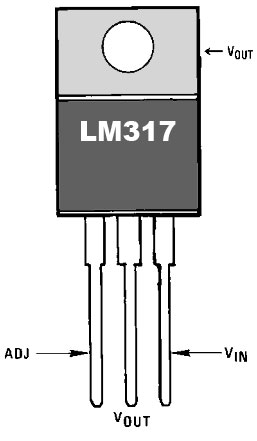
\includegraphics[width=1in]{lm317}
	\caption{Pin out of the LM317 IC.}
	\label{fig:lm317}
\end{figure}

A linear regulator provides very stable and clean voltage output but it can only provide regulated output voltage lower than the primary voltage source. Another disadvantage of a linear regulator is its low efficiency when the difference between the input and output voltages is large. Because the same amount of current flows through the regulator and the load, the power being dissipated is roughly

\begin{equation}
	P_d=I_{load} \times \left( V_{in}-V_{out}\right).
\end{equation}

When the load current is high, this power dissipation can be significant. It is therefore important to provide good heat sinking to the regulator IC. In fact, many regulator ICs, such as the LM317, have large exposed metal pad with low thermal resistance to facilitate mounting a heat sink.  However, it is very important to note that the metal pad on some regulator ICs, such as the LM317, is connected electrically to the output of the IC. If the heat sink may potentially come in contact with any other part of the circuit (including the enclosure, which often is tied to ground), proper isolation is needed between the IC and the heat sink. 
%
%When choosing a linear voltage regulator, several important specifications should be considered:
%\begin{itemize}[itemsep=0.5ex]
%	\item \textbf{Output voltage range}: the amount of ;
%	\item Maximum output current;
%	\item Drop-out voltage: this is the smallest voltage difference between the input and the output voltage before the output is no longer regulated. Having a low drop-out voltage is often advantageous;
%	\item Load regulation: the change in output voltage for a given change in load current;
%	\item Line regulation: the change in output voltage for a given input voltage change. 
%\end{itemize}

\begin{enumerate}
\item Using Fig.~\ref{fig:lm317_lab} as a reference, build the regulator circuit on the breadboard. You should be able to find the LM317 pinout diagram from its datasheet, which you find from online. \emph{As a general suggestion, it is important to keep your circuit well laid out and keep the connecting wires as short as possible. Cut the wires to the right length if necessary.} Fig.xxx shows an example breadboard layout for the LM317 regulator circuit in this lab. 

	\begin{figure}[h]
	\centering
		\begin{circuitikz}[scale=1]
				\centering	
				\draw (-2,0) node [above]{$V_{in}$} to [short,o-] (1,0)
				(-1,0) to [C, l=$C_i${=}\SI{0.1}{\micro\farad}] (-1,-2) node [sground]{}
				(1,-0.5) rectangle (3,0.5)
				(1.4,0.1) node [scale=0.75]{V$_{\text{IN}}$}
				(2,0.75) node []{LM317}
				(2.55,0.1) node [scale=0.75]{V$_{\text{OUT}}$}
				(2,-0.3) node [scale=0.75]{ADJ}
				(3,0) to (3.5,0) to [R, l=$R_1${=}\SI{220}{\ohm}] (3.5,-2) to (2,-2)
				(2,-0.5) to (2,-2) to [vR, l=$R_2: \text{2K potentiometer}$] (2,-4) node [sground]{}
				(3.5,0) to [short, -o] (7,0) node [above]{$V_{out}$}
				(6,0) to [C, l=$C_o${=}\SI{1}{\micro\farad}] (6,-2) node [sground]{}
				;
			\end{circuitikz}
		\caption{Schematic of the voltage regulator circuit using LM317.}
		\label{fig:lm317_lab}
	\end{figure}
	
	\begin{figure}[h]
		\centering
		\includegraphics[width=1in]{lm317-board}
		\caption{.}
		\label{fig:lm317-board}
	\end{figure}


\item For testing the circuit, we will first use the lab bench power supply as our input power. Set the power supply voltage to 8\,V and connect it to the input of your voltage regulator circuit. Adjust the $R_2$ potentiometer until the output voltage is 5\,V. You can use the lab multimeter to measure the output voltage. 

\item Line regulation: 
	\begin{enumerate}
		\item Adjust the input voltage from 8\,V to 5\,V at 0.25\,V intervals, and then from 5\,V to 2\,V at 0.5\,V intervals, record the regulator output voltage using the multimeter; 
		\item Plot your results. In what input voltage range does the LM317 provide good line regulation? 
		\item What is the dropout voltage at various input voltages? Does it agree with the datasheet?
	\end{enumerate}
	
% load regulation:

\end{enumerate}

\subsection{Precision voltage reference}

In order to present a precise and stable reference for the DAC and the ADC, we will build a precision voltage reference circuit. In this circuit, we will use the TI LT1009 reference IC with 2.5\,V output voltage and less than $\pm$ 0.2\% initial accuracy (no calibration and adjustment). The LT1009 IC can be used as a two-terminal voltage reference although it does provide an optional 3rd terminal for $\pm 5$\% adjustment.

\begin{enumerate}
	\item Build circuit shown in Fig. on your breadboard.
	 
	\begin{figure}[h]
	\centering
		\begin{circuitikz}[scale=0.75]
				\centering	
				\draw (0,0) node[ground] {} to [full Zener diode, l=LT1009] (0,2) to [R,l=\SI{3.6}{\kilo \ohm}] (0,4) to (0,4.5) node[above]{5\,V}
				(0,2) to [short,*-o] (2,2) node[right]{$V_{REF}$}
				;
			\end{circuitikz}
		\caption{Schematic of the LT1009 precision voltage reference circuit.}
		\label{fig:lm317_lab}
	\end{figure}
	
	\item Verify that the output voltage of the circuit is 2.5\,V.
\end{enumerate}

\subsection{Function generator}

There are numerous ways to build a function generator. You can use a 555 timer, a ring of inverters, dedicated oscillator ICs, or a direct digital synthesis (DDS) circuit which uses high-speed digital circuits to implement fast waveform generators. It does so by outputting values from a look-up table (LUT), which stores the desired waveform in discretized values, and converting them to an analog signal by a DAC. 

In this lab, we will try to emulate a DDS using a micro-controller and an MCP4921 DAC. We are interested in generating a triangle wave which will be useful in later labs. Since DAC outputs are discrete in nature, we are really just approximating the triangle wave with a stair-case waveform (Fig.~\ref{fig:triangle-wave}). Obviously, the higher the resolution of the DAC, the better this approximate is. 

For this class, we will use the \textit{Teensy 3.1} micro-controller. The Teensy 3.1 is developed by Paul J.~Stoffregen of \href{https://www.pjrc.com}{PJRC.com}. The programming of Teensy 3.1 is done in the same IDE as the Arduino platform\footnote{with an add-on called Teensyduino, which has already been installed on the lab computer} and most Arduino programs will run without any problem on the Teensy. Compared to most Arduinos, however, the Teensy 3.1 has a much faster micro-controller (72\,MHz, overclockable to 144\,MHz) with floating point support and is therefore a much better platform than Arduinos when some number crunching is needed. 

	\begin{figure}[h]
		\centering
		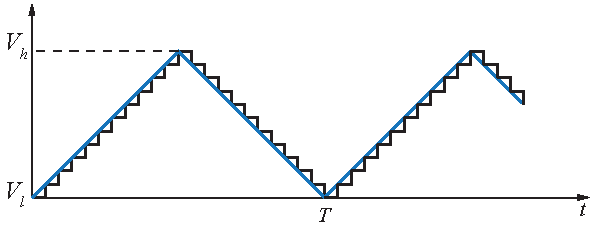
\includegraphics[width=4in]{triangle-wave}
		\caption{Triangle wave and its approximation by a stair-case waveform which more closely resembles the output of a DAC.}
		\label{fig:triangle-wave}
	\end{figure}


\begin{enumerate}
	\item Using Fig.~\ref{fig:uno_sch} as a reference, connect the Teensy to the MCP4921 DAC. Connect the MCP4921's VDD pin to the output of the LM317 regulator (5\,V). Connect the MCP4921's VREF pin to the LT1009 reference's output (2.5\,V). Connect both AVSS and $\overline{\text{LDAC}}$ of the MCP4921 to ground. A \SI{0.1}{\micro\farad} and a \SI{1}{\micro\farad} capacitor could be used at VREF to minimize noise at the reference. It is very important to keep your circuit (ICs, resistors, capacitors, wires, etc) organized. Use as short of a wire as possible between two connection points. Refer to Fig.~\ref{fig:uno_pic} for an example layout.
	


	\begin{figure}[h]
	\centering
		\begin{circuitikz}
				\centering	
				\draw (2, 0) rectangle (5,5)
				;
			\end{circuitikz}
		\caption{Schematic of the connection between Arduino UNO and the MCP4921.}
		\label{fig:uno_sch}
	\end{figure}


\item Once the circuit is built, open the Arduino IDE, create a new sketch, and input the code \href{https://github.com/ucdart/UCD-EEC134/blob/master/Lab1/triangle.ino}{``triangle\_teensy\_mcp4921.ino''} . \textbf{Make sure you read through and understand the code.} You may also want to read the datesheet of MCP4921 to understand its SPI control protocol. 

\item Connect the Teensy with the computer using a USB cable, which is used to power up and program the Teensy.

\item Compile and upload the code to the Teensy. Use the following settings under the ``Tools'' menu: 
	\begin{enumerate}
		\item Board: ``Teensy 3.1''
		\item USB Type: ``Serial''
		\item CPU Speed: ``144\,MHz Optimized (Overclocked)''
	\end{enumerate}

\item In your report, include a screen capture of both the triangle (at VOUTA) and sync (at SYNC) output signals on the oscilloscope. Record their amplitudes and periods.

\item Modify your code to set the triangle wave amplitude to 2.5\,V. Hint: change the gain setting of the MCP4921. 

\item How can you modify the code to change the amplitude and period of the output waveform? What is the fastest triangle wave you could generate? What do you think is the limitation to going even faster?

\item Modify the code to generate a sinusoidal wave. What is the highest frequency sinusoidal wave you can generate? The following link may give you some hint. 
\url{http://interface.khm.de/index.php/lab/experiments/arduino-dds-sinewave-generator/} 

%\item \textbf{(Challenge!)} Research and propose a design that will allow you to generate a 100\,kHz triangle and/or sine wave. (Hint: look-up table)

\item The Teensy actually has a built-in DAC. Try to implement the triangle wave generator using the built-in DAC. Refer to \url{https://www.pjrc.com/teensy/teensy31.html} for some hint. What is the fastest triangle wave you can generate?

\item Use code \href{https://github.com/ucdart/UCD-EEC134/blob/master/labs/lab1/code/triangle_teensy_audio/triangle_teensy_audio.ino}{``triangle\_teensy\_audio.ino''} to generate a 4\,kHz sine wave using Teensy's built in DAC. The code makes use of the \href{http://www.pjrc.com/teensy/td_libs_Audio.html}{Teensy Audio library}. You should dig into the \href{https://github.com/PaulStoffregen/Audio}{source code}, in particular the \href{https://github.com/PaulStoffregen/Audio/blob/master/synth_waveform.cpp}{``synth\_waveform.cpp''} file, of the audio library to understand how it works. 
\end{enumerate}

\subsection{Low-pass filter}

In this part of the lab, we will implement an active low pass filter (LPF) with an adjustable gain stage. In the final radar system, the LPF+Gain stage will be responsible for filtering out spurious signals that may disturb the received baseband radar signals. We will use the Texas Instrument OPA4228 quad Op-Amp for both the gain stage and the active LPF. A pinout diagram of OPA4228 is shown in Fig. 6.10.4. Fig.~\ref{fig:lpf_sch} shows the schematic of the circuit. Fig.~\ref{fig:lpf_pic} shows an example of the actual circuit on a breadboard. 

The filter has a cut-off frequency of 15\,kHz. 

%It also filters out any spurious signals above a certain threshold frequency (15\,kHz in this design). To get the maximum resolution from the digitizer, the maximum strength of the signal should be less than the allowed input voltage range of the digitizer. 

%In our simple radar system, we are going to use the soundcard of the PC as the digitizer. The amplified and filtered IF signal is fed to the right channel of an audio card, which is conventionally connected using the red wire of a 3.5\,mm stereo jack or the ring of the connector (Fig. 6.10.3). 

\begin{figure}[h]
	\centering
	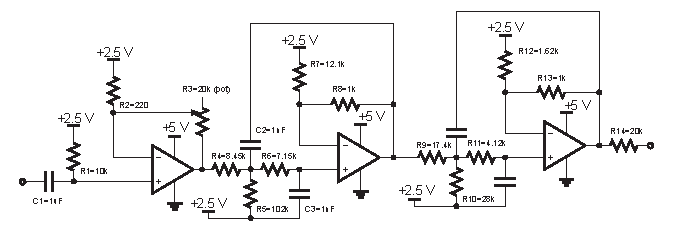
\includegraphics[width=5in]{lpf_sch}
	\caption{Schematic of the active low-pass filter.}
	\label{fig:lpf_sch}
\end{figure}



\subsubsection{Gain stage}

\begin{enumerate}

	\item Identify the gain stage of the audio amplifier from Fig. xxx. What is the expression of its gain? Notice the +2.5\,V bias does not affect this result, rather it simply shifts the bias of the overall amplifier since a single 5\,V supply (battery) is used vs a dual-rail (both positive and negative) supply.
	
	\item Build the gain stage on your breadboard. 
		\begin{enumerate}
			\item Power the op-amp chip by using 5\,V for VDD and ground for VSS. You may use the LM317 regulator or the USB battery  pack to provide the 5\,V. It's a good idea to disconnect and turn off the battery pack when measurement is not being made.
			
			\item You can use the 2.5\,V LT1009 reference as the bias for the input and output. 
			
			\item The gain is controlled using a 20\,k\si{\ohm} potentiometer (POT). 			
		\end{enumerate}

	\item To test the circuit, generate a 1\,kHz 30\,mVpp sine wave signal using the lab signal generator and connect the signal to the input of the gain stage circuit. Measure the output of the circuit using the lab oscilloscope. What is the maximum peak-to-peak voltage at the output before clipping occurs? What is the gain at this point?
	
	\item Tabulate and plot the gain from 100\,Hz to 1\,MHz while keeping the pot fixed. Find the 3\,dB cutoff frequency or the 3\,dB bandwidth at this gain. Use at least 20 data points.
	
%The audio card on a typical laptop is designed to take in line level signals. Notice that this limits the sound card input signal strength to approximately 3\,Vpp. Adjust the pot to achieve 3\,Vpp on the oscilloscope at 1 kHz. 

\end{enumerate}

\subsubsection{Active LPF}
Build the rest of the audio amplifier circuit, i.e. the active LPF. To measure just the filter response, disconnect R4 and R14 from the circuit (Fig. 6.10.1). Input a 3\,Vpp signal in place of R4 and measure the output in place of R14. R14 will only be needed as a current limiting resistor when connecting the amplifier to the laptop’s audio card. Again tabulate and plot the frequency response from 100 Hz to 20 kHz. What is the cutoff frequency of the filter?
The overall filter consists of 2 low pass filters. What is the order of the overall filter and how is it determined from the schematic? Is the bandwidth of the filter tunable? How would one increase or decrease the cutoff frequency?
What limitation does the cut-off frequency of the LPF place on the radar’s performance?  (Hint: what happens when your object is too far away)

\subsubsection{Gain Stage + Filter}
\begin{enumerate}
	\item Reconnect R4 (R14 is still disconnected) and measure the overall response of the amplifier. Input a 100\,mVpp sine wave to the IF input. 
	
	\item Adjust the pot for a 3\,Vpp output at 1\,kHz and once again sweep the frequency from 100\,Hz to 20\,kHz while tabulating the voltage output and the gain. What is the cutoff frequency? Compare the results to previous measurements. Tabulate and plot all of the results for the report.
	
	\item Reconnect R14. Break the audio cable and connect the LPF output to the right channel and the SYNC signal (from the modulator) to the left channel. 
		
\end{enumerate}


\subsection{Analog-to-digital converter}

\subsection{Signal processing}

Use teensy 3.1 to sample and process data? sounds like too much work...

Using the laptop

\subsection{PCB Design}

\begin{thebibliography}{9}

\bibitem{lamport94}
  Leslie Lamport,
  \emph{\LaTeX: a document preparation system},
  Addison Wesley, Massachusetts,
  2nd edition,
  1994.

\end{thebibliography}

\end{document}